\section{Testing}
\label{sec:testing}

In order to get some preliminary results to verify whether or not this is a good approach for crashproofing HDF5, we identified two metadata-intensive benchmarks (A and B) and one non-metadata-heavy benchmark (C): 
\begin{itemize}
    \item Benchmark A: generates an HDF5 file of size 135 MB and a total of 77,111 metadata writes.
    \item Benchmark B: generates an HDF5 file of size 23 GB and a total of 1,821,278 metadata writes.
    \item Benchmark C: generates an HDF5 file of size 41 MB and a total of 66 metadata writes.
 \end{itemize}

\begin{center}
\begin{tabular}{|c|c|c|c|}
\hline
   benchmark & file size & metadata writes \\
   \hline
   A  & 135 MB & 77,111 \\
   \hline
   B & 23 GB & 1,821,278\\
   \hline
   C & 41 MB & 66\\
   \hline
\end{tabular}
\end{center}
 
We then modified the library's MPIO driver to write the address and size of all the metadata writes to a log file $M$.

A dummy WAL writer was created to read the log file $M$, and for each piece of metadata read, write the metadata address, size, and bytes equal to the size of the metadata of random data to a dummy WAL file. This is meant to simulate the writing of actual metadata into a WAL file down the line.

To determine the overhead from occasional HDF5 file syncs, which are necessary for a \textit{Log Checkpoint}, we modified the library's MPIO driver to flush the HDF5 file intermittently based on the amount of metadata written. The time needed for the HDF5 file syncs was also recorded to see if it would be problematic to keep the WAL file small for metadata heavy applications.

The same thing was done for the dummy WAL writer. Since the dummy WAL writer would need to handle both \textit{Log Flush }and \textit{Log Checkpoint}, we added the ability to flush every $x$ bytes to simulate a \textit{Log Flush} to help sync the playback location and the ability to trim and flush the file every $y$ bytes to simulate a \textit{Log Checkpoint} to help reduce the size of the WAL.

For runs with no \textit{Log Checkpoint}, the flush interval has no effect on the modified MPIO file driver, and hence we used the results from a single set of averaged runs for all flush interval cases. For Benchmark C, the dummy WAL writer does not contribute a significant amount of time to the result, hence the results for Benchmark C with only \textit{Log Flush} show the same result for all flush intervals.

Specifically, we tested:
\begin{itemize}
    \item A \textit{Log Flush} every 64 KB and a \textit{Log Checkpoint} every 1 MB
    \item A \textit{Log Flush} every 256 KB and a \textit{Log Checkpoint} every 4 MB
    \item A \textit{Log Flush} every 1 MB and a\textit{Log Checkpoint} every 16 MB
    \item A \textit{Log Flush} every 4 MB and a \textit{Log Checkpoint} every 64 MB
    \item A \textit{Log Flush} every 16 MB and a \textit{Log Checkpoint} every 256 MB
    \item A \textit{Log Flush} every 64 KB
    \item A \textit{Log Flush} every 256 KB
    \item A \textit{Log Flush} every 1 MB
    \item A \textit{Log Flush} every 4 MB
    \item A \textit{Log Flush} every 16 MB
\end{itemize}

The preliminary results for benchmark A \& B indicated that:
\begin{itemize}
    \item The overhead for \textit{Log Flush} + \textit{Log Checkpoint} both decrease as we increase the interval at which we perform HDF5 file syncs.
    \item The overhead for \textit{Log Flush} is minimal, and mostly comes from adding an HDF5 file sync before file close.
\end{itemize}
See the graphs below for more information.

Note the X-axis for the graphs list the \textit{Log Checkpoint} interval, even for runs with only \textit{Log Flush}. The \textit{Log Flush} interval is always as listed above for the corresponding specified \textit{Log Checkpoint} interval.

% testing - matt
\begin{center}
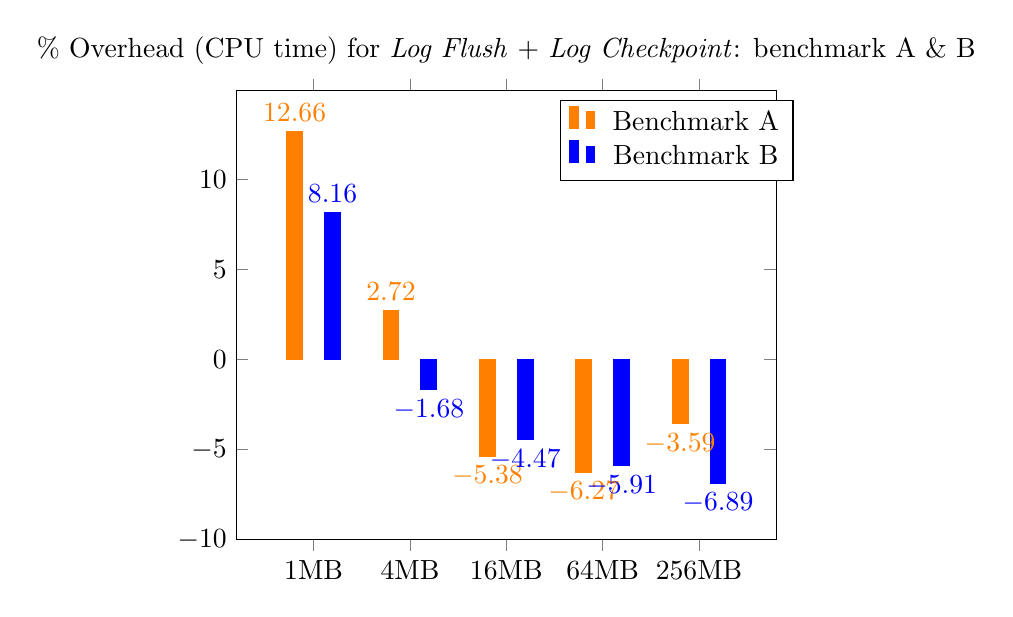
\begin{tikzpicture}
\begin{axis}
[
title=\% Overhead (CPU time) for \textit{Log Flush} + \textit{Log Checkpoint}: benchmark A \& B,
ybar=8pt,
nodes near coords,
bar width=0.2cm,
ymin=-10,
symbolic x coords={1MB,4MB,16MB,64MB,256MB},
xtick=data,
enlarge x limits=.2,
   legend style={
      at={(.6,.8)}, 
      anchor=south west,
      column sep=1ex
}
]
\addplot[style={orange,fill=orange}]
         coordinates{(1MB,12.657)(4MB,2.721)(16MB,-5.380)(64MB,-6.267)(256MB,-3.587)};
\addplot[style={blue,fill=blue}]
         coordinates{(1MB,8.155)(4MB,-1.679)(16MB,-4.474)(64MB,-5.907)(256MB,-6.893)};    
\addlegendentry[mark color=orange]{Benchmark A}
\addlegendentry[mark color=blue]{Benchmark B}
\end{axis}
\end{tikzpicture}
\end{center}

\begin{center}
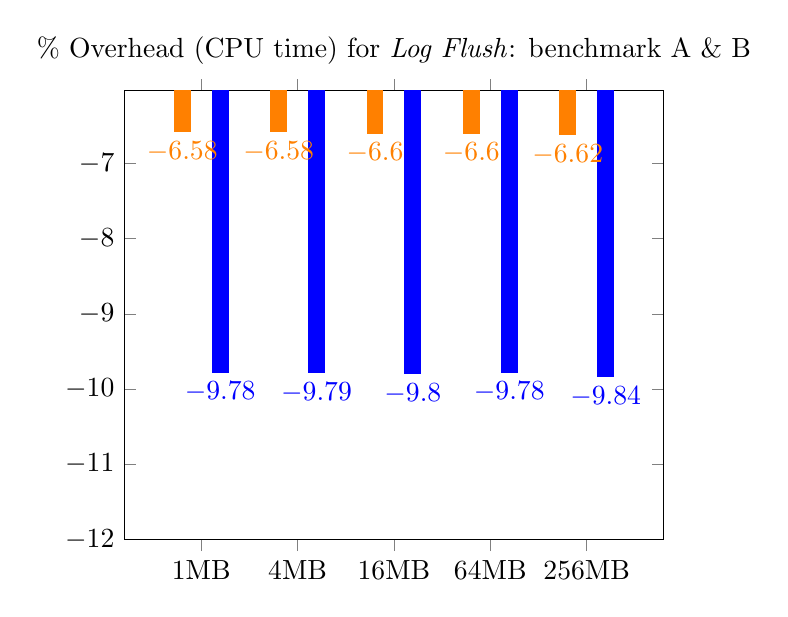
\begin{tikzpicture}
\begin{axis}
[
title=\% Overhead (CPU time) for \textit{Log Flush}: benchmark A \& B,
ybar=8pt,
nodes near coords,
bar width=0.2cm,
ymin=-12,
symbolic x coords={1MB,4MB,16MB,64MB,256MB},
xtick=data,
enlarge x limits=.2,
   legend style={
      at={(.6,.8)}, 
      anchor=south,
      column sep=1ex
}
]
\addplot[style={orange,fill=orange}]
        coordinates{(1MB,-6.576)(4MB,-6.576)(16MB,-6.597)
        (64MB,-6.597)(256MB,-6.617)};
\addplot[style={blue,fill=blue}]
        coordinates{(1MB,-9.779)(4MB,-9.785)(16MB,-9.799)
        (64MB,-9.779)(256MB,-9.838)};      
\end{axis}
\end{tikzpicture}
\end{center}

\begin{center}
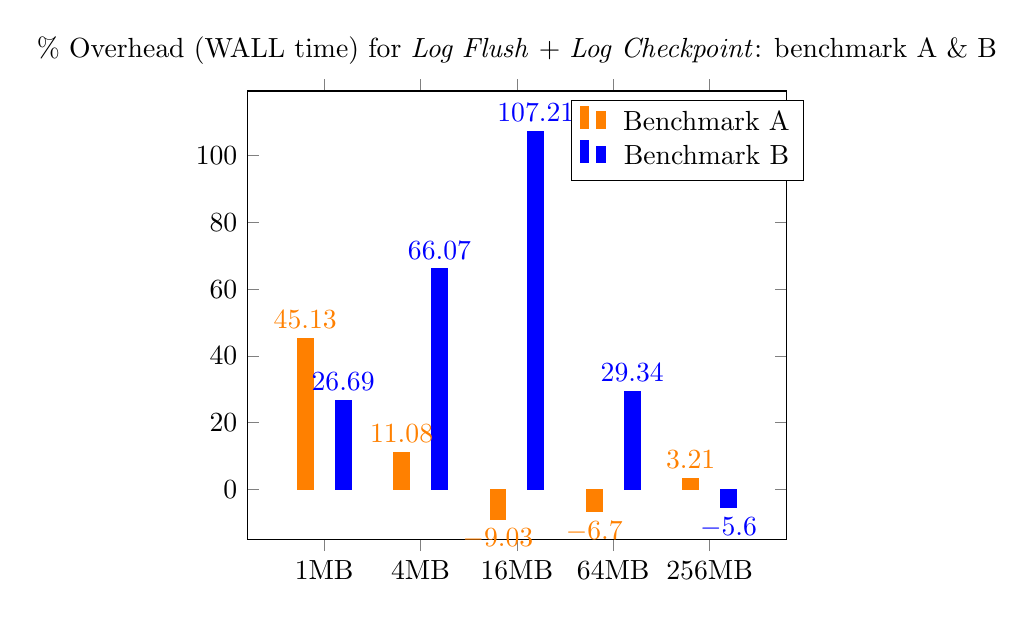
\begin{tikzpicture}
\begin{axis}
[
title=\% Overhead (WALL time) for \textit{Log Flush} + \textit{Log Checkpoint}: benchmark A \& B,
ybar=8pt,
nodes near coords,
bar width=0.2cm,
ymin=-15,
symbolic x coords={1MB,4MB,16MB,64MB,256MB},
xtick=data,
enlarge x limits=.2,
   legend style={
      at={(.6,.8)}, 
      anchor=south west,
      column sep=1ex
}
]
\addplot[style={orange,fill=orange}]
        coordinates{(1MB,45.129)(4MB,11.076)(16MB,-9.029)
        (64MB,-6.702)(256MB,3.210)};
\addplot[style={blue,fill=blue}]
        coordinates{(1MB,26.691)(4MB,66.066)(16MB,107.205)(64MB,29.342)(256MB,-5.604)};   
\addlegendentry[mark color=orange]{Benchmark A}
\addlegendentry[mark color=blue]{Benchmark B}
\end{axis}
\end{tikzpicture}
\end{center}

\begin{center}
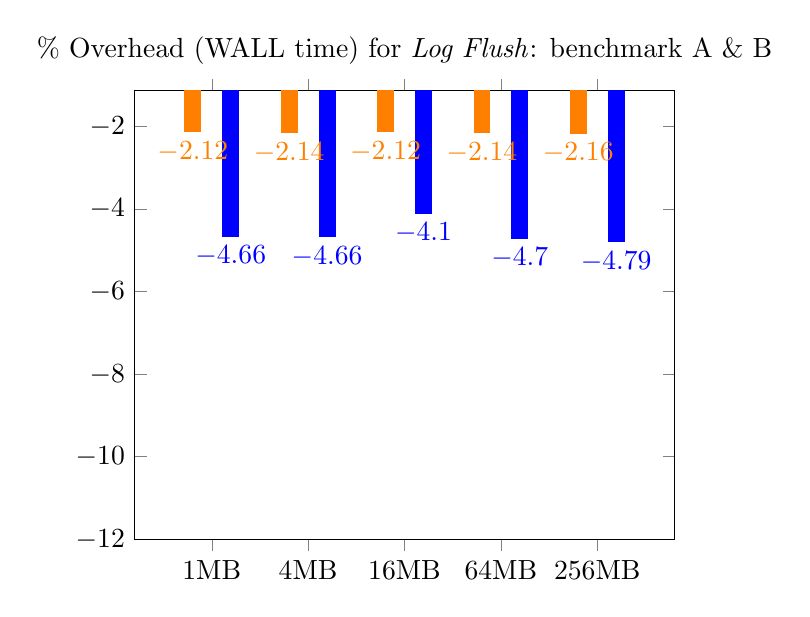
\begin{tikzpicture}
\begin{axis}
[
title=\% Overhead (WALL time) for \textit{Log Flush}: benchmark A \& B,
ybar=8pt,
nodes near coords,
bar width=0.2cm,
ymin=-12,
symbolic x coords={1MB,4MB,16MB,64MB,256MB},
xtick=data,
enlarge x limits=.2,
   legend style={
      at={(.6,.8)}, 
      anchor=south,
      column sep=1ex
}
]
\addplot[style={orange,fill=orange}]
        coordinates{(1MB,-2.121)(4MB,-2.140)(16MB,-2.121)
        (64MB,-2.140)(256MB,-2.159)};
\addplot[style={blue,fill=blue}]
        coordinates{(1MB,-4.657)(4MB,-4.659)(16MB,-4.095)
        (64MB,-4.697)(256MB,-4.789)};   
\end{axis}
\end{tikzpicture}
\end{center}

As for benchmark C, the four graphs below indicated that the overhead for \textit{Log Flush} as well as \textit{Log Flush} + \textit{Log Checkpoint} is minimal.

\begin{center}
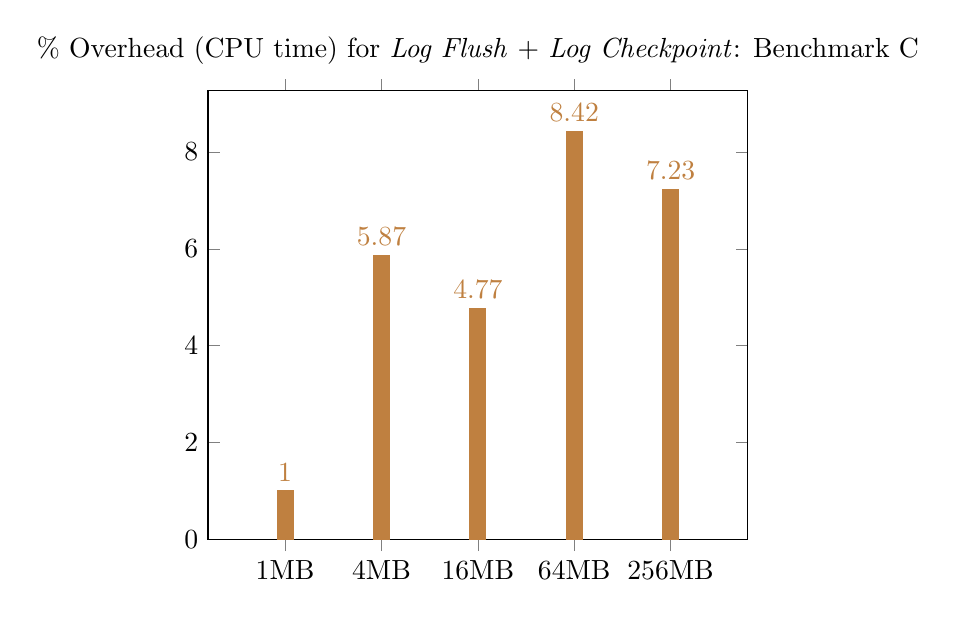
\begin{tikzpicture}
\begin{axis}
[
title=\% Overhead (CPU time) for \textit{Log Flush} + \textit{Log Checkpoint}: Benchmark C,
ybar=8pt,
nodes near coords,
bar width=0.2cm,
ymin=0,
symbolic x coords={1MB,4MB,16MB,64MB,256MB},
xtick=data,
enlarge x limits=.2,
   legend style={
      at={(.6,.8)}, 
      anchor=south,
      column sep=1ex
}
]
\addplot[style={brown,fill=brown}]
        coordinates{(1MB,0.998)(4MB,5.869)(16MB,4.771)
        (64MB,8.421)(256MB,7.230)};
\end{axis}
\end{tikzpicture}
\end{center}

\begin{center}
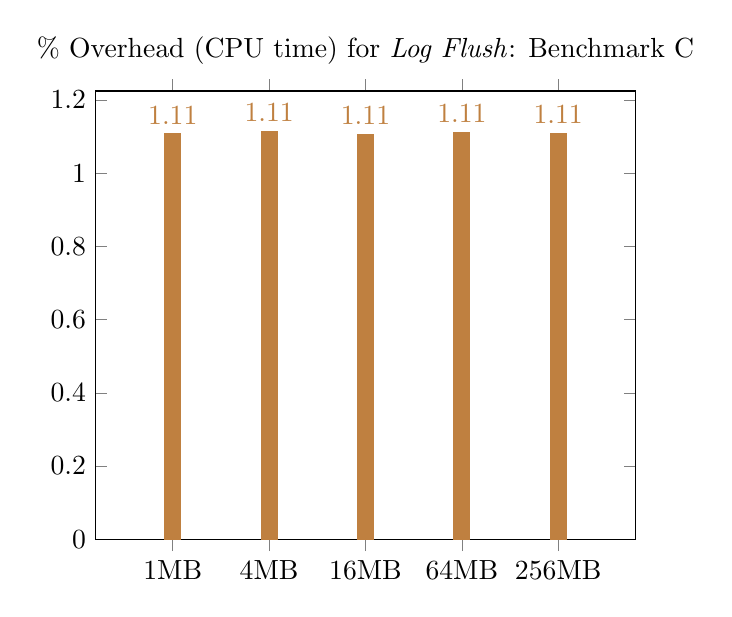
\begin{tikzpicture}
\begin{axis}
[
title=\% Overhead (CPU time) for \textit{Log Flush}: Benchmark C,
ybar=8pt,
nodes near coords,
bar width=0.2cm,
ymin=0,
symbolic x coords={1MB,4MB,16MB,64MB,256MB},
xtick=data,
enlarge x limits=.2,
   legend style={
      at={(.6,.8)}, 
      anchor=south,
      column sep=1ex
}
]
\addplot[style={brown,fill=brown}]
         coordinates{(1MB,1.107)(4MB,1.113)(16MB,1.105)
         (64MB,1.112)(256MB,1.108)}; 
\end{axis}
\end{tikzpicture}
\end{center}

\begin{center}
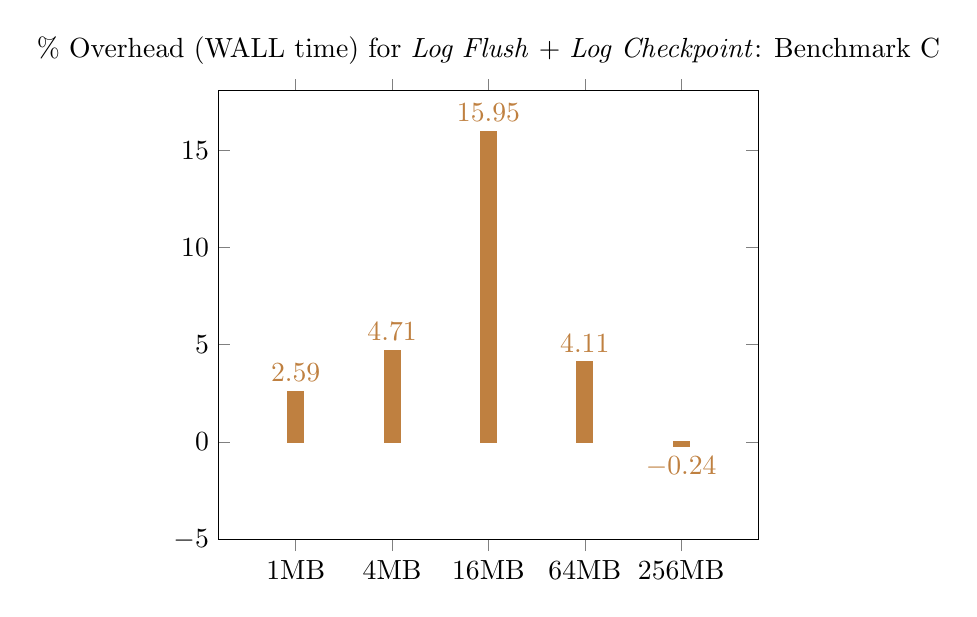
\begin{tikzpicture}
\begin{axis}
[
title=\% Overhead (WALL time) for \textit{Log Flush} + \textit{Log Checkpoint}: Benchmark C,
ybar=8pt,
nodes near coords,
bar width=0.2cm,
ymin=-5,
symbolic x coords={1MB,4MB,16MB,64MB,256MB},
xtick=data,
enlarge x limits=.2,
   legend style={
      at={(.6,.8)}, 
      anchor=south,
      column sep=1ex
}
]
\addplot[style={brown,fill=brown}]
         coordinates{(1MB,2.591)(4MB,4.714)(16MB,15.948)
         (64MB,4.111)(256MB,-0.235)};       
\end{axis}
\end{tikzpicture}
\end{center}

\begin{center}
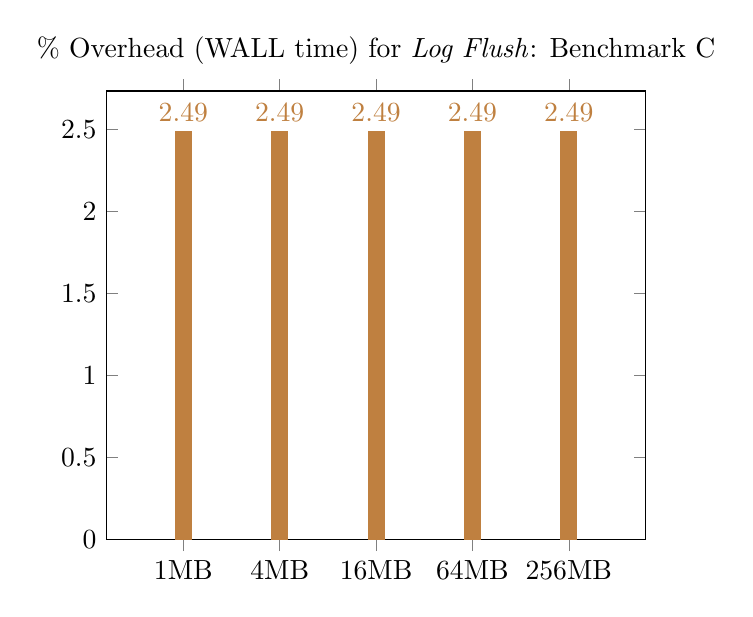
\begin{tikzpicture}
\begin{axis}
[
title=\% Overhead (WALL time) for \textit{Log Flush}: Benchmark C,
ybar=8pt,
nodes near coords,
bar width=0.2cm,
ymin=0,
symbolic x coords={1MB,4MB,16MB,64MB,256MB},
xtick=data,
enlarge x limits=.2,
   legend style={
      at={(.6,.8)}, 
      anchor=south,
      column sep=1ex
}
]
\addplot[style={brown,fill=brown}]
         coordinates{(1MB,2.487)(4MB,2.487)(16MB,2.487)
         (64MB,2.487)(256MB,2.487)}; 
\end{axis}
\end{tikzpicture}
\end{center}

The following four graphs (CPU and WALL time) report the overhead for \textit{Log Flush} as well as \textit{Log Flush} + \textit{Log Checkpoint} when running benchmark C with a larger file size (167MB) and 4 ranks.

\begin{center}
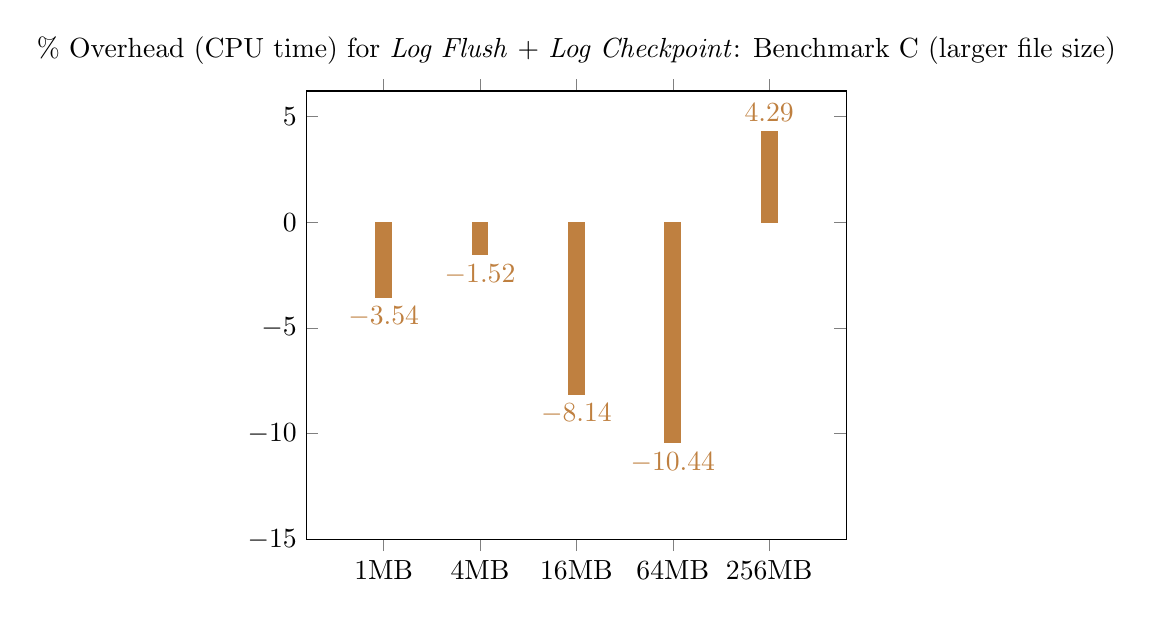
\begin{tikzpicture}
\begin{axis}
[
title=\% Overhead (CPU time) for \textit{Log Flush} + \textit{Log Checkpoint}: Benchmark C (larger file size),
ybar=8pt,
nodes near coords,
bar width=0.2cm,
ymin=-15,
symbolic x coords={1MB,4MB,16MB,64MB,256MB},
xtick=data,
enlarge x limits=.2,
   legend style={
      at={(.6,.8)}, 
      anchor=south,
      column sep=1ex
}
]
\addplot[style={brown,fill=brown}]
        coordinates{(1MB,-3.538)(4MB,-1.517)(16MB,-8.139)
        (64MB,-10.438)(256MB,4.290)};
\end{axis}
\end{tikzpicture}
\end{center}

\begin{center}
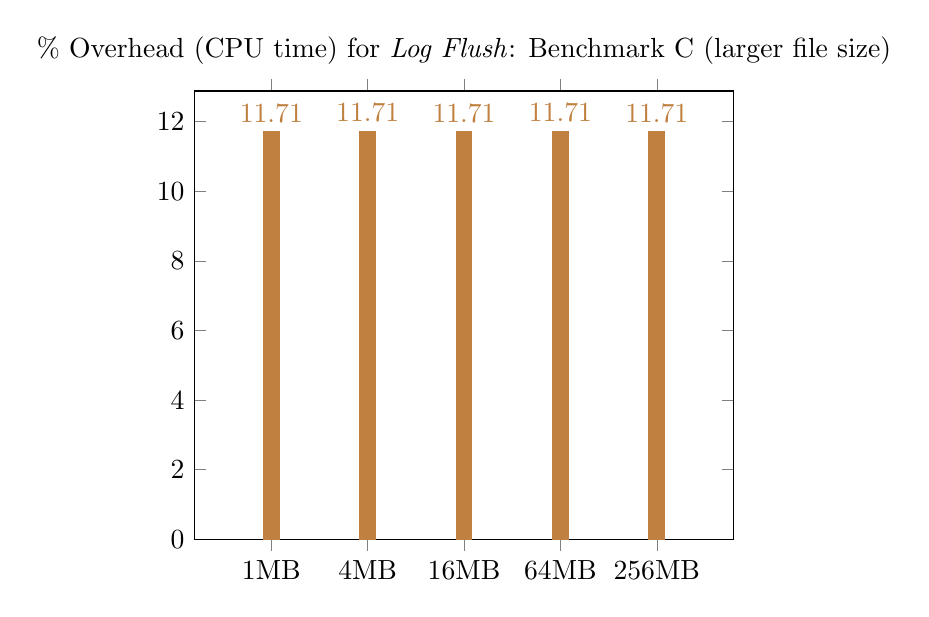
\begin{tikzpicture}
\begin{axis}
[
title=\% Overhead (CPU time) for \textit{Log Flush}: Benchmark C (larger file size),
ybar=8pt,
nodes near coords,
bar width=0.2cm,
ymin=0,
symbolic x coords={1MB,4MB,16MB,64MB,256MB},
xtick=data,
enlarge x limits=.2,
   legend style={
      at={(.6,.8)}, 
      anchor=south,
      column sep=1ex
}
]
\addplot[style={brown,fill=brown}]
         coordinates{(1MB,11.712)(4MB,11.714)(16MB,11.711)
         (64MB,11.713)(256MB,11.712)}; 
\end{axis}
\end{tikzpicture}
\end{center}

\begin{center}
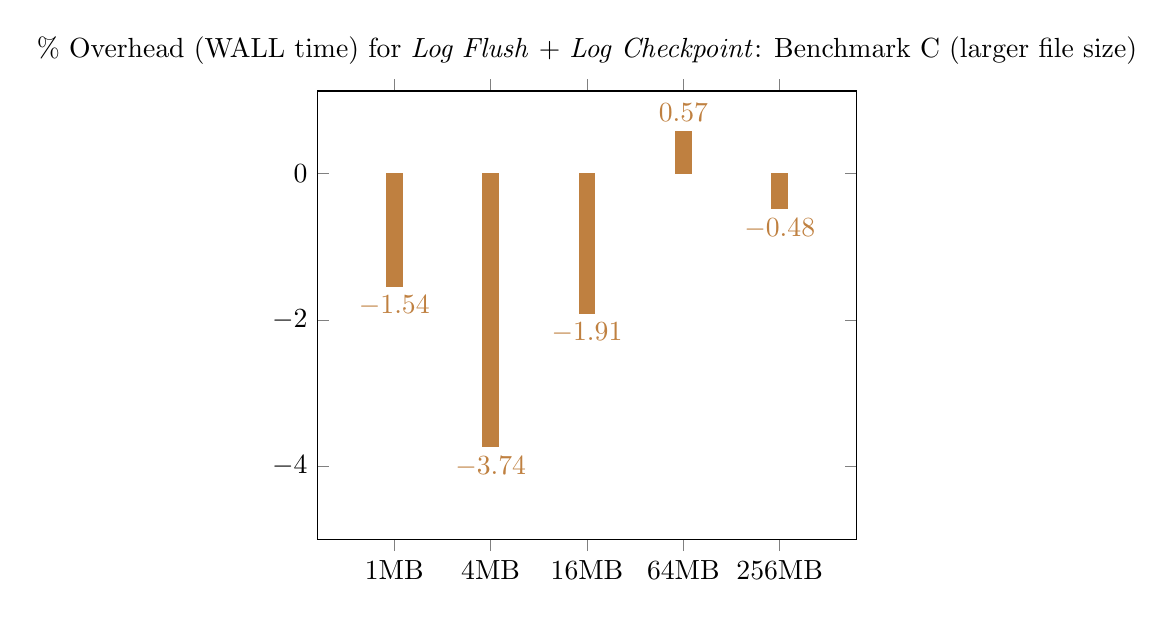
\begin{tikzpicture}
\begin{axis}
[
title=\% Overhead (WALL time) for \textit{Log Flush} + \textit{Log Checkpoint}: Benchmark C (larger file size),
ybar=8pt,
nodes near coords,
bar width=0.2cm,
ymin=-5,
symbolic x coords={1MB,4MB,16MB,64MB,256MB},
xtick=data,
enlarge x limits=.2,
   legend style={
      at={(.6,.8)}, 
      anchor=south,
      column sep=1ex
}
]
\addplot[style={brown,fill=brown}]
        coordinates{(1MB,-1.537)(4MB,-3.737)(16MB,-1.908)
        (64MB,0.573)(256MB,-0.483)};
\end{axis}
\end{tikzpicture}
\end{center}

\begin{center}
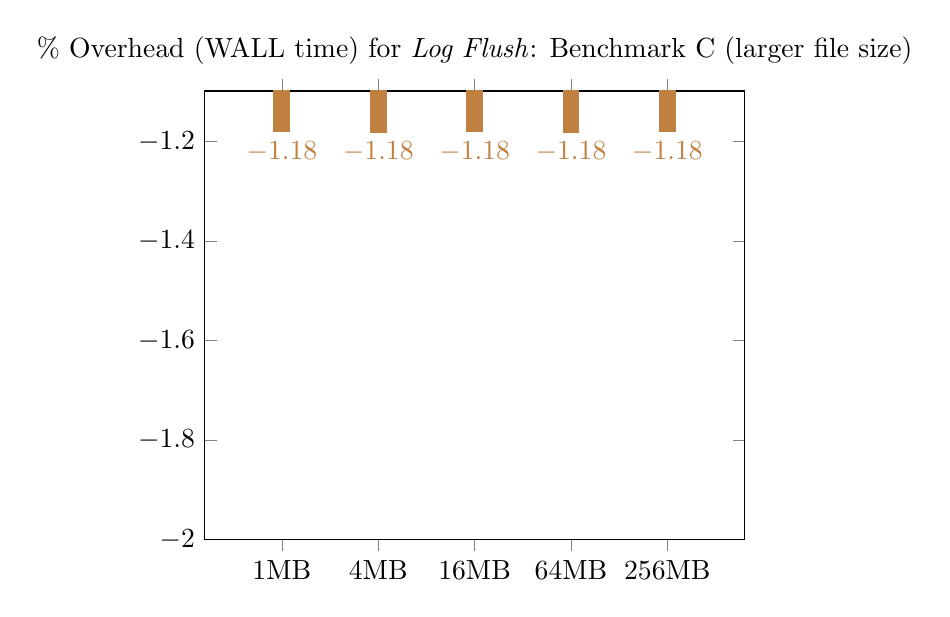
\begin{tikzpicture}
\begin{axis}
[
title=\% Overhead (WALL time) for \textit{Log Flush}: Benchmark C (larger file size),
ybar=8pt,
nodes near coords,
bar width=0.2cm,
ymin=-2,
symbolic x coords={1MB,4MB,16MB,64MB,256MB},
xtick=data,
enlarge x limits=.2,
   legend style={
      at={(.6,.8)}, 
      anchor=south,
      column sep=1ex
}
]
\addplot[style={brown,fill=brown}]
         coordinates{(1MB,-1.180)(4MB,-1.181)(16MB,-1.180)
         (64MB,-1.181)(256MB,-1.180)}; 
\end{axis}
\end{tikzpicture}
\end{center}